% Created with jtex v.1.0.20
\documentclass{article}
\PassOptionsToPackage{short, nodayofweek}{datetime}


% Start Curvenote Definitions

% Pass Options Section
% base
\PassOptionsToPackage{normalem}{ulem}
\PassOptionsToPackage{utf8}{inputenc}

% template
\PassOptionsToPackage{framemethod=TikZ}{mdframed}
\PassOptionsToPackage{x11names, svgnames}{xcolor}

%%% PACKAGES

% base
\usepackage{inputenc}
\usepackage{url}
\usepackage{graphicx}
\usepackage{adjustbox}
\usepackage{amssymb}
\usepackage{amsfonts}
\usepackage{amsmath}
\usepackage{enumitem}
\usepackage{nicefrac}
\usepackage{booktabs}
\usepackage{microtype}
\usepackage{hyperref}
\usepackage{ulem}
\usepackage{enumitem}
\usepackage{float}
\usepackage{datetime}
\usepackage{xkeyval}
\usepackage{framed}
\usepackage{doi}

% template
\usepackage{natbib}
\usepackage{fancyvrb}
\usepackage{mdframed}
\usepackage{xcolor}

%%%


%%%% Setup Section

% base
\graphicspath{{.}}
% template
\sloppy
\newenvironment{aside}{\begin{framed}}{\end{framed}}
\newmdenv[linewidth=2pt,linecolor=CornflowerBlue,topline=false,bottomline=false,rightline=false,leftline=true,skipabove=20,skipbelow=20,leftmargin=20,rightmargin=20]{callout}
\newfloat{code}{thp}{loc}
\floatname{code}{Program}
\raggedbottom
\bibliographystyle{abbrvnat}
\setcitestyle{authoryear,open={(},close={)},semicolon,aysep={,}}

% End Curvenote Definitions




% colors for hyperlinks
\hypersetup{colorlinks=true, allcolors=blue}
\hypersetup{
pdftitle={\@title},
pdfsubject={},
pdfauthor={\@author},
pdfkeywords={},
addtopdfcreator={Written in Curvenote}
}

\usepackage{curvenote}

\title{Ch. 4: Using EMG to measure muscle fatigue}

\newdate{articleDate}{17}{2}{2025}
\date{\displaydate{articleDate}}

\author{\bfseries Erin McKiernan\mdseries\\Universidad Nacional Autónoma de México (UNAM), Open Research Community Accelerator (ORCA)\\\AND\bfseries Saúl A. Saldaña Enciso\mdseries\\}

\begin{document}

\maketitle
\keywords{}

\section{Overview}

In this experimental practical, students learn about the physiological mechanisms underlying muscle fatigue, including the different types of motor units and muscle fibers, their characteristics, and their contributions to contractions of varying force. Students explore how to activate and tire their muscles in different ways, and how to detect changes in the EMG signal that indicate fatigue. Overall, this practical is designed to help students understand more about the function of skeletal muscle, and how fatigue is related to both electrical activity and the biochemical and physiological properties of muscle cells. The duration of this practical can vary from 1-2 hours for a single session, or multiple sessions if the experiment is more complex and involves various volunteers to be compared. While not necessary, it is recommended that students carry out the experimental practical in \href{https://curvenote.com/oxa:EPpXta8zJdzN048lz8AR/hZTnTYzQR5EQmCKX51Wj}{Ch. 1: Muscle physiology and EMG basics }prior to this practical.

\section{Learning objectives}

\textbf{Before} this practical, students should:

\begin{itemize}
\item understand the basics of cellular metabolism, including glycolysis and cellular respiration
\item understand the basics of how skeletal muscles function and how contractions are produced (for review, see Chapter 1 in this e-book)
\item know how electrical activity is generated in muscle and the basics of EMG recording (recommended that students carry out the practical in Chapter 1)
\item be able to define the different types of contractions see in muscle
\end{itemize}

\textbf{During} this practical, students will:

\begin{itemize}
\item further explore the use of EMG recording to measure muscle activity, paying special attention to changes in amplitude and frequency
\item compare and contrast how different types of contractions (isotonic, concentric, eccentric, isometric, etc.) produce fatigue in muscle
\item investigate performing contractions with and without weight to produce fatigue
\item observe any differences in fatigue in sustained versus repeated contractions
\end{itemize}

\textbf{After} this practical, students should be able to:

\begin{itemize}
\item describe what happens to the EMG recording as muscles fatigue
\item explain the underlying physiological mechanisms that produce this fatigue, and correspondingly, why this induces changes in the EMG signal
\item design additional experiments to explore fatigue in other muscles
\end{itemize}

\section{Equipment and materials}

\begin{itemize}
\item \href{https://backyardbrains.com/products/muscle-spikerbox}{Muscle SpikerBox} (Backyard Brains)
\item 9V battery to power SpikerBox
\item Round surface electrodes (any medical supply provider)
\item Cable with alligator clips to connect electrodes to SpikerBox (Backyard Brains)
\item Cable to connect SpikerBox to a computer, tablet, or phone (Backyard Brains)
\item Computer, tablet, or phone with free Backyard Brains \href{https://backyardbrains.com/products/byb-spike-recorder}{Spike Recorder software} installed
\item Computer, tablet, or phone adaptor, 3.5mm aux to USB-C (if no aux port on devices; any provider)
\item Alcohol and cotton swabs to clean skin (if necessary) before recording, and to help remove electrodes after recording (optional)
\item Dumbbells or other objects to perform muscle loading (e.g. books, backpacks); if these are of known mass, this will help to control the level of fatigue
\item Other indications: Wear loose clothing to permit electrode placement, and be careful not to overload muscles to avoid injury
\end{itemize}

\section{Background information}

\subsection{Motor units and their characteristics}

The process of excitation-contraction coupling that we saw in Chapter 1 begins when a motor neuron (MN) sends electrical impulses to the muscle fibers it innervates \citep{schneider2012skeletal, openStax_muscle}. This functional collection of one MN and its synaptically connected muscle fibers is called a motor unit \citep{}Figure \%s ``. Muscles contain multiple motor units of different sizes and types. It is the coordinated activity of these units that allows muscles to generate contractions of varying force and duration.

\begin{figure}[!htbp]
\centering
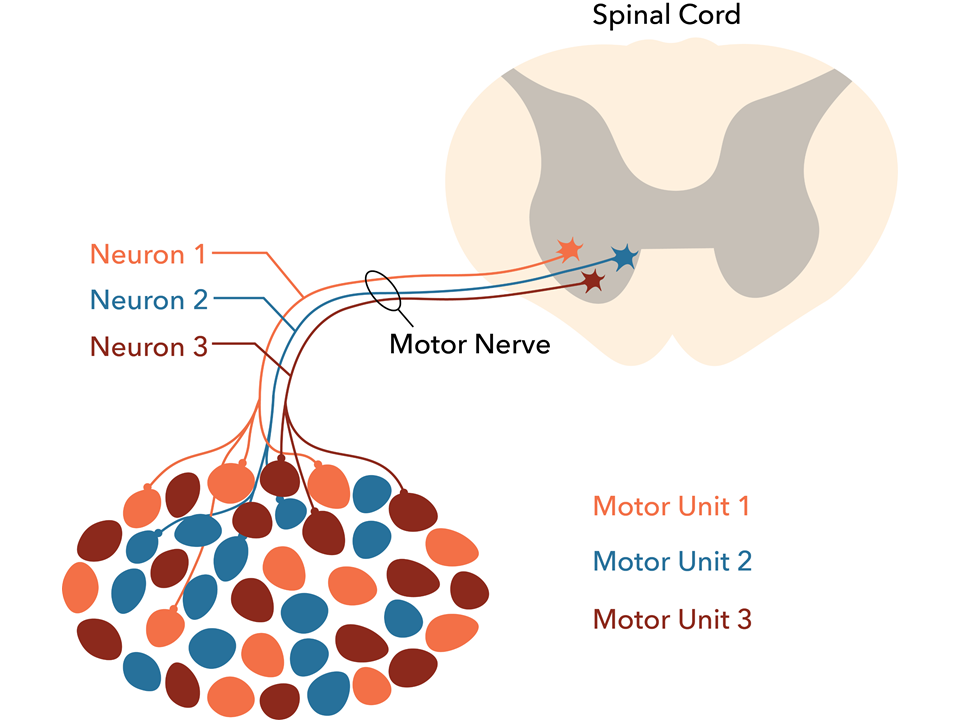
\includegraphics[width=0.7\linewidth]{files/EPpXta8zJdzN048lz8AR-ea5a4a1e321179708726b68563d91c8a.png}
\caption[]{Motor neurons, whose somas are seen here in a transversal slice of the spinal cord, extend their nerves to innervate different muscles fibers (color coded). Each MN and its innervated fibers constitutes a motor unit. Image credit: Daniel Walsh \& Alan Sved, CC BY-SA 4.0, via Wikimedia Commons \href{https://upload.wikimedia.org/wikipedia/commons/1/1b/Motor\_unit.png}{https://upload.wikimedia.org/wikipedia/commons/1/1b/Motor\_unit.png}}
\label{FpL67ayhha}
\end{figure}

Motor units (MUs) can vary in size, both with respect to the diameter of the MN soma (cell body) and the total number of fibers innervated. As \citet{Dideriksen2013Motor} point out, these factors are correlated, since ``the size of the soma of a motor neuron is associated to the diameter of its axon\dotsand the axon diameter determines the degree to which the axon divides into terminal branches''. In other words, smaller MNs tend to innervate fewer muscle fibers than larger MNs. As we will see below, the size of a MU is an important factor in its recruitment and its participation in force generation.

MUs also differ with respect to other characteristics, apart from just their size, including their contractile features and metabolic capabilities \citep{Weinberger2010} . Generally, MUs are divided into three types: slow fatigue-resistant (Type I or S), fast fatigue-resistant (Type IIa or FR), and fast fatigable (Type IIb or FF). Type I MUs are smaller and generate the least amount of force. However, they can maintain prolonged contractions (i.e. they hardly fatigue) due to an abundance of mitochondria in the muscle fibers, allowing them to create energy through oxidative (aerobic) metabolism. Type IIa MUs generate more force than Type I's and are still somewhat resistant to fatigue due to a decent number of mitochondria and good perfusion that allows them to also use oxidative metabolism. In contrast, Type IIb MUs generate the largest force, but are highly susceptible to fatigue since their low mitochondrial numbers and poor perfusion means they depend instead on glycolytic (anaerobic) metabolism. Muscles vary in the overall balance of these different MU types, depending on their functions (posture versus power) and the forces or contraction speeds they need to produce. For example, studies have found that certain extraocular muscles (e.g. orbicularis oculi) contain primarily fast fatigable (Type IIb) units or fibers \citep{tong2024anatomy}, while certain leg muscles (e.g soleus) contain mostly slow (Type I) fibers \citep{Weinberger2010}. This, in turn affects their relative contractions times (Figure~\ref{WuEQUeZj3K} ).

\begin{figure}[!htbp]
\centering
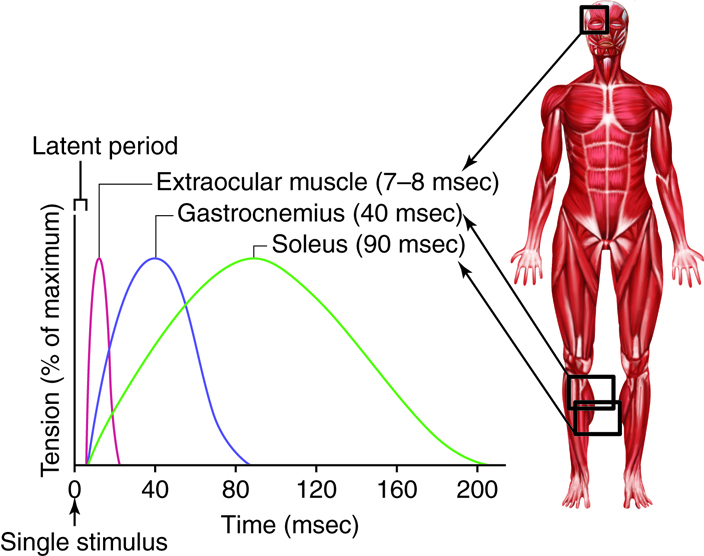
\includegraphics[width=0.7\linewidth]{files/EPpXta8zJdzN048lz8AR-d9dc00d816c074c6bec6802c66922e89.jpeg}
\caption[]{Muscle contraction times in different muscles as measured by electromyography in response to electrical stimulation. Image credit: \href{https://commons.m.wikimedia.org/wiki/File:Electromyograph\_of\_muscle\_twitch\_responses.jpg}{https://commons.m.wikimedia.org/wiki/File:Electromyograph\_of\_muscle\_twitch\_responses.jpg}}
\label{WuEQUeZj3K}
\end{figure}

\subsubsection{Study question}

\begin{enumerate}
\item How will knowing the above --- i.e. that some muscles are designed for short, forceful contractions, while others are meant for sustained, postural contractions --- affect your experimental design?
\end{enumerate}

\subsection{Motor unit recruitment and force generation}

The size of a motor unit determines the order in which it is recruited during contractions. Smaller MNs have a larger input resistance, and thus respond with larger membrane depolarizations when stimulated, i.e. smaller synaptic currents can induce them to fire action potentials (APs). As a consequence, when muscle contraction begins, the first motor units to be recruited are the smallest ones, followed by increasingly larger units as force increases. This is known as the Size Principle, or Henneman's Principle, after the scientist who first described this phenomenon in detail \citep{Mendell2005size}. However, because of their small size and the fewer number of muscle fibers innervated, a presynaptic potential from a Type I (or S) MN results in a much smaller postsynaptic twitch amplitude in the muscle than that generated by the large Type II (or F) units \citep{}Figure \%s ``. So, there is an inverse relationship between recruitment order and twitch amplitude (i.e. force generation).

\begin{figure}[!htbp]
\centering
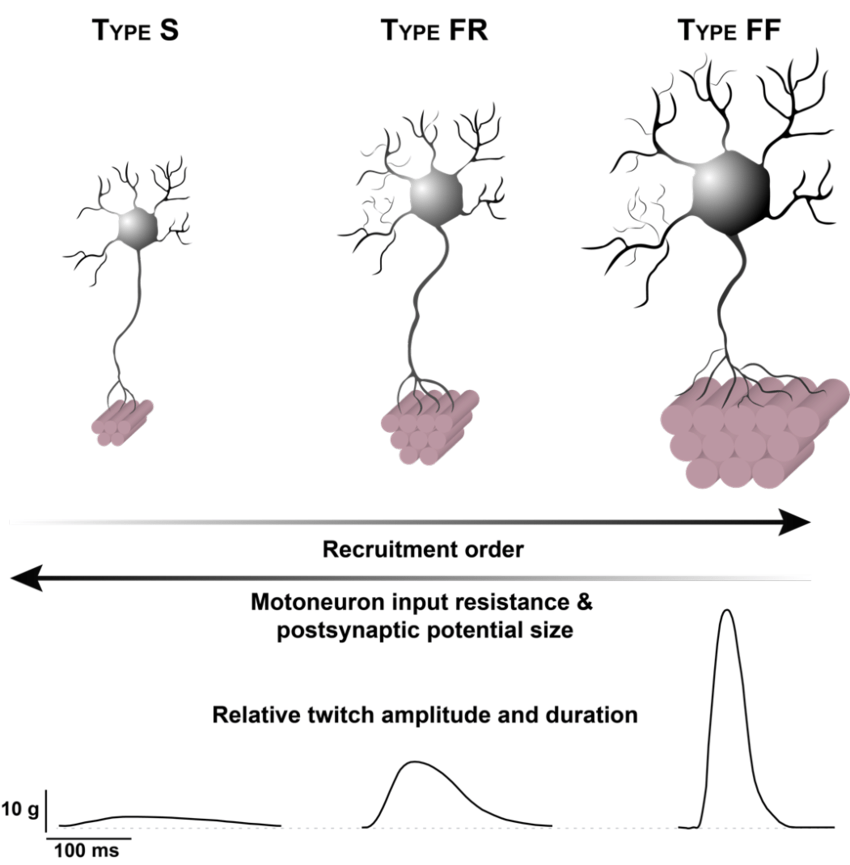
\includegraphics[width=0.7\linewidth]{files/EPpXta8zJdzN048lz8AR-0d4b04daf13968f2c348204e34c11d3e.png}
\caption[]{``A simplified depiction of motor unit types that comprise a continuum. Motor units are grouped according to their size, which primarily determines their recruitment order. As size of the parent motoneuron increases, so does the number and size of innervated muscle fibers.'' From Pearcey \& Rymer, CC BY-NC-ND, Available: \href{https://www.researchgate.net/figure/A-simplified-depiction-of-motor-unit-types-that-comprise-a-continuum-Motor-units-are\_fig1\_362943933}{https://www.researchgate.net/figure/A-simplified-depiction-of-motor-unit-types-that-comprise-a-continuum-Motor-units-are\_fig1\_362943933}}
\label{d88kUpTUVw}
\end{figure}

In accordance with the characteristics of small versus large MUs that we saw in Section~\ref{AFAVfbwQAj}, the Size Principle also means that we first recruit the Type I (slow oxidative) fibers, followed by Type IIa (fast oxidative), and then finally Type IIb (fast glycolytic) fibers as tension in the muscle approaches maximum. As we can see in Figure~\ref{jSKUh8ycDq}, while they are recruited first, Type I MUs contribute more to sustaining a low baseline level of tension in the muscle, while larger units come in later to provide larger but shorter `boosts' when additional power is needed. The difference in force generation between Type I and Type II MUs can be up to 100 fold \citep{Weinberger2010}.

Why do we see these functional differences in MUs and how are these related to their biophysical properties and metabolic processes? First, the speed of tension development is directly proportional to the rate of ATP hydrolysis in the muscle fibers during cross-bridge cycling (see Ch. 1 for review of this cycle, the main `players', and its energy requirements). Type I fibers express a type (isoform) of myosin which has a slower rate of ATP hydrolysis than the isoform expressed in Type II fibers \citep{biga} . This, in turn limits the rate at which actin and myosin can interact in Type I fibers and thereby makes contraction slower. Second, the source of ATP in muscle fibers is important. As we learned in Section~\ref{AFAVfbwQAj}, Type I and Type IIa fibers use oxidation (i.e. cellular respiration), while Type IIb fibers use glycolysis. The former metabolic process produces at least 15 times the quantity of ATP produced by the latter, thereby providing a much larger source of energy for contraction \citep{biava}.

\begin{figure}[!htbp]
\centering
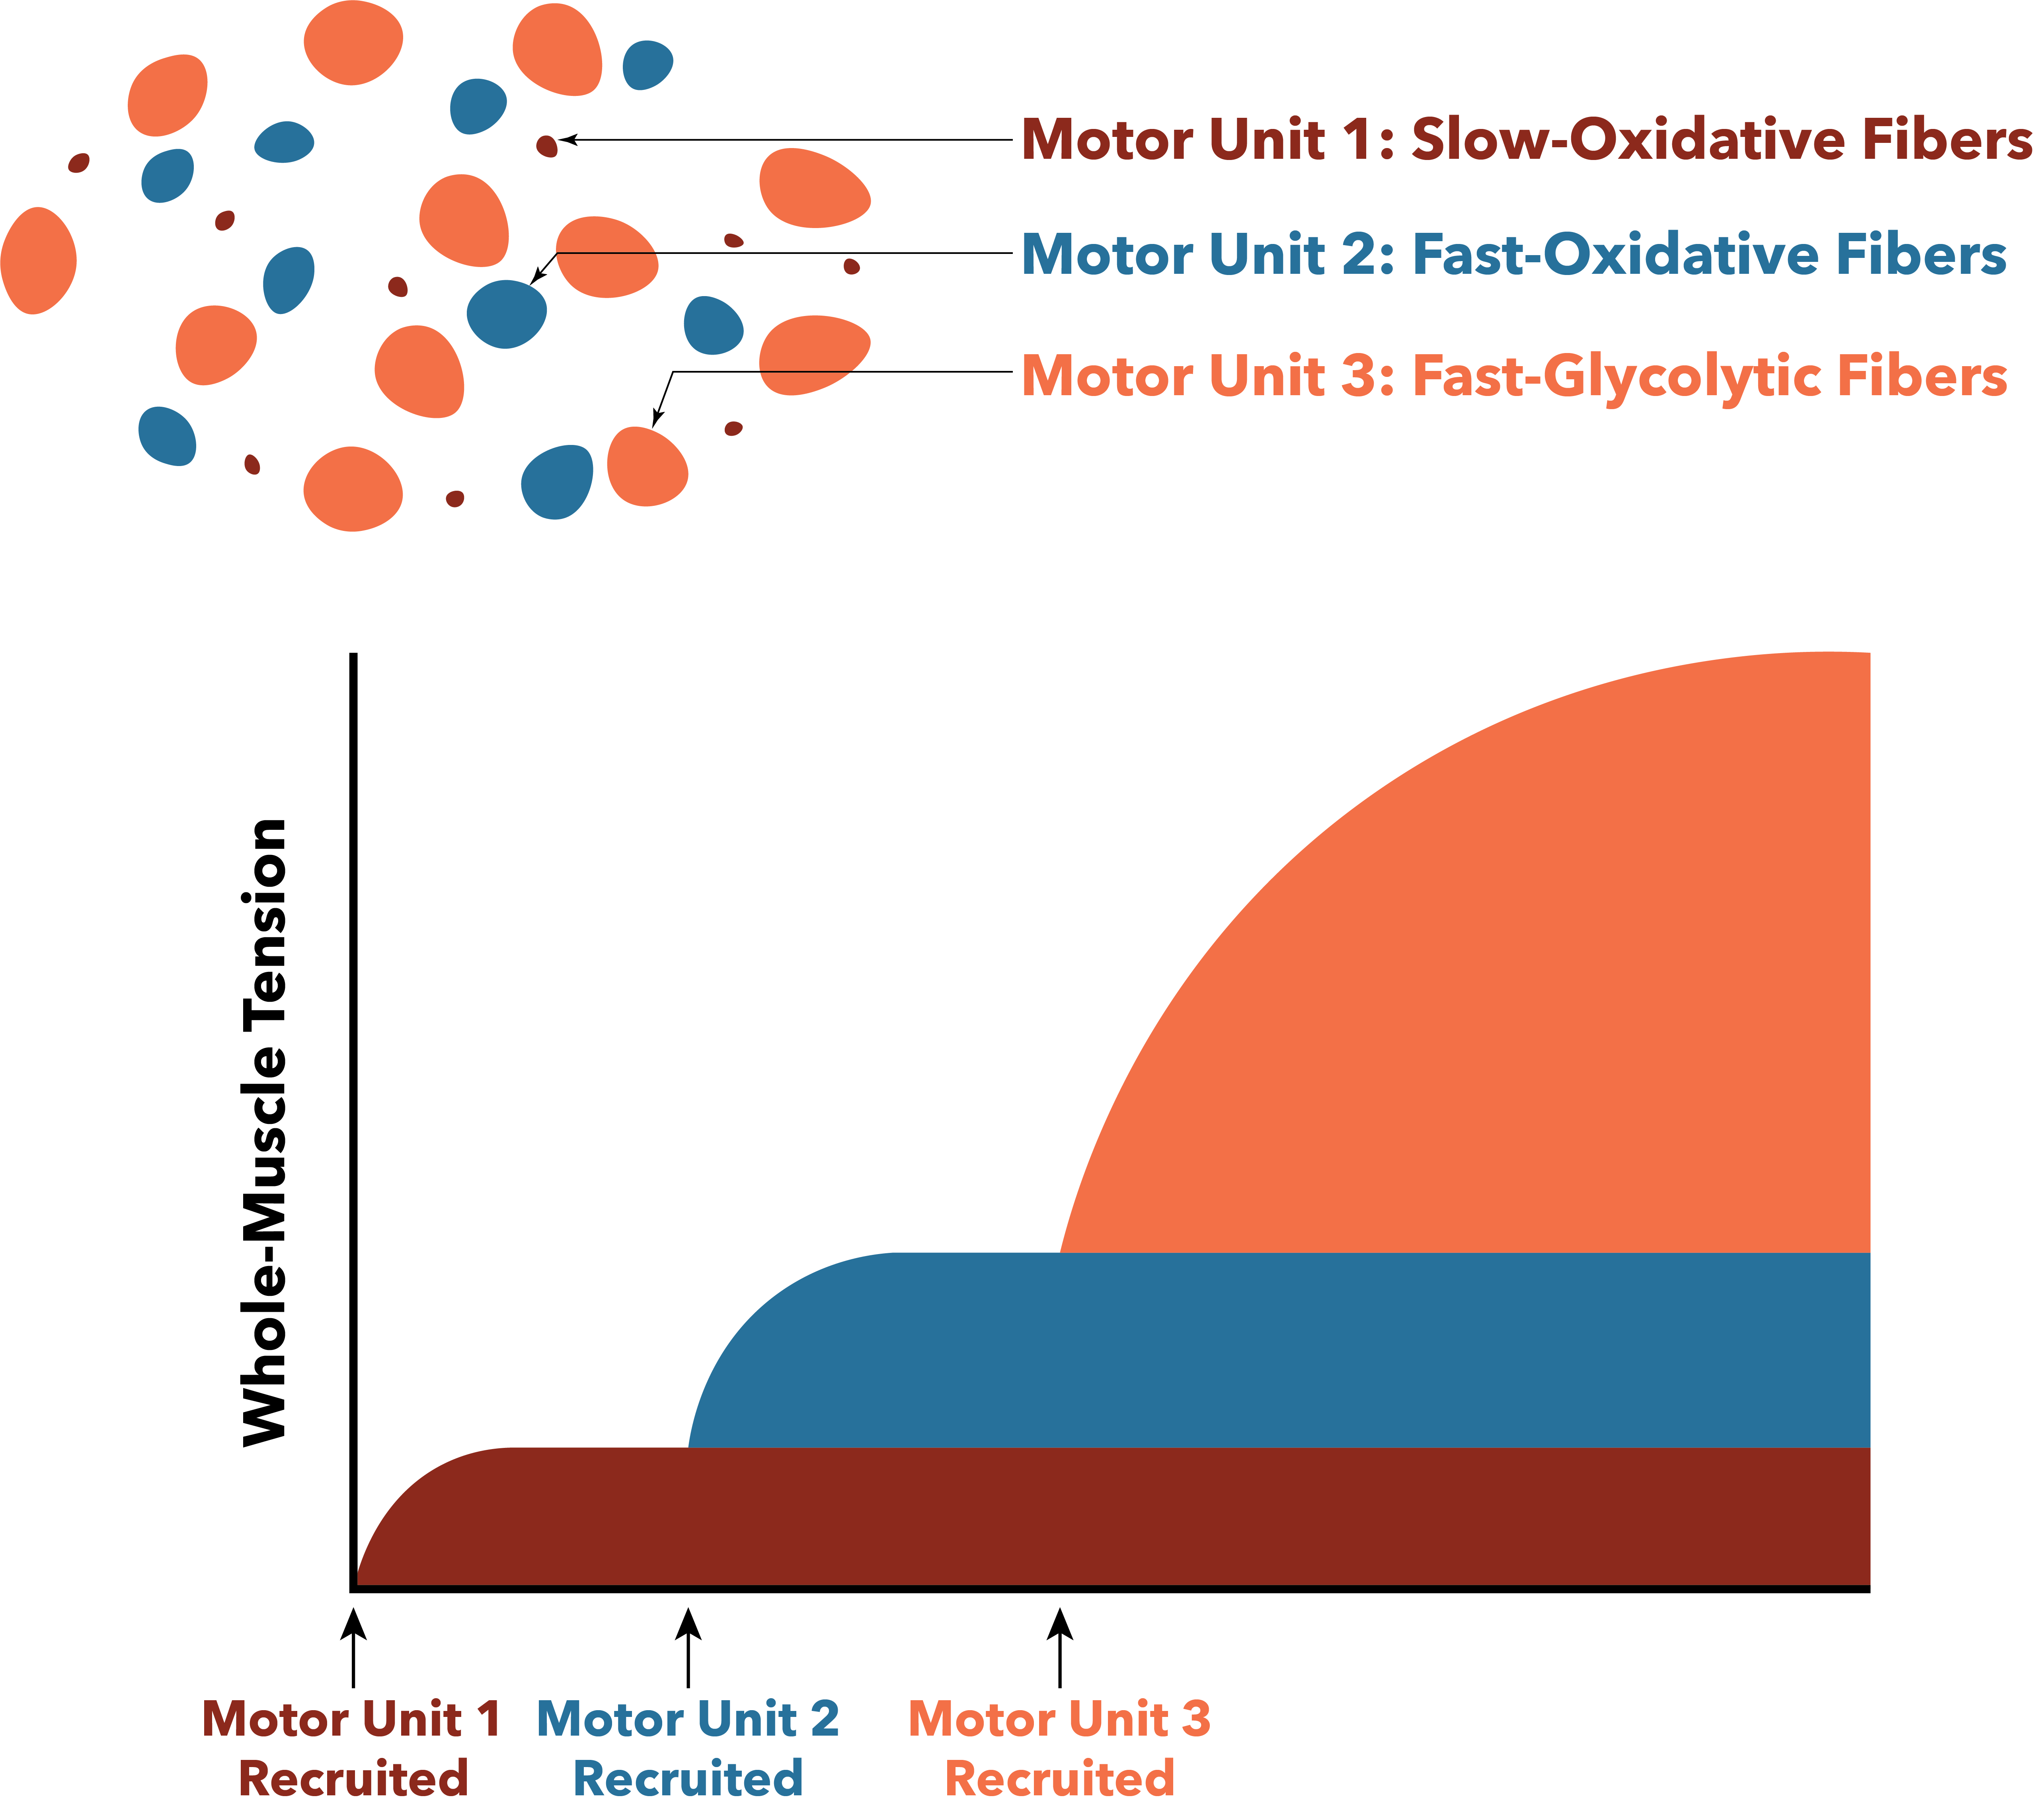
\includegraphics[width=0.7\linewidth]{files/EPpXta8zJdzN048lz8AR-6c5448b34ae723d7ef83e4bd325a35f6.png}
\caption[]{Different sizes and types of motor units (above) are recruited depending on the force/tension needed (below). At the lowest level of tension, only the small and slow (Type I) units are recruited. As the larger, fast (Type IIa and IIb) units are recruited, more tension can be produced. Image credit: Daniel Walsh and Alan Sved, CC BY-SA 4.0, via Wikimedia Commons \href{https://upload.wikimedia.org/wikipedia/commons/7/73/Motor\_unit\_recruitment.png}{https://upload.wikimedia.org/wikipedia/commons/7/73/Motor\_unit\_recruitment.png}}
\label{jSKUh8ycDq}
\end{figure}

\subsection{Sources and mechanisms of fatigue}

\citet{enoka2008muscle} write that ``the term muscle fatigue is used to denote a transient decrease in the capacity to perform physical actions''. However, due to potential issues with this, they say ``most investigators invoke a more focused definition of muscle fatigue as an exercise-induced reduction in the ability of muscle to produce force or power whether or not the task can be sustained''. They go on to clarify, ``Accordingly, muscle fatigue is not the point of task failure or the moment when the muscles become exhausted. Rather, muscle fatigue is a decrease in the maximal force or power that the involved muscles can produce, and it \textbf{develops gradually soon after the onset of the sustained physical activity}'' (emphasis added). So, what happens at the level of the MU (both within the MN and the muscle fibers) that causes this gradual decrease in force?

\subsubsection{At the muscle level}

The properties of muscle fibers reviewed in the above sections and summarized in Figure~\ref{n9KlNIgbBP} have direct implications for understanding muscle fatigue. If we ask a person to contract a muscle of interest and generate as much force as they can, called the Maximum Voluntary Contraction (MVC), we will see that the electromyogram (EMG) initially shows a strong signal with large amplitude, high-frequency electrical potentials. However, eventually, both the amplitude and frequency of the signal begin to decrease \citep{georgiou2017microelectronics} as MUs which are susceptible to fatigue `drop out' of the recording. The first to go will be the Type IIb (fast fatigable) MUs, since the reliance of these fibers on glycolytic metabolism does not provide sufficient energy to sustain their activity. The longer a contraction goes on, the more Type IIb units will drop out, followed subsequently by Type IIa (fast fatigue resistant) MUs. While IIa fibers can sustain contraction for longer than IIb fibers, they still have fewer mitochondria than Type I fibers and depend at least partially on glycolytic metabolism \citep{Weinberger2010}. Eventually, if the contraction lasts long enough, only Type I MUs will be left. In this way, force is diminished over time as the muscle fibers capable of generating larger tension successively cease to contribute to force.

\begin{figure}[!htbp]
\centering
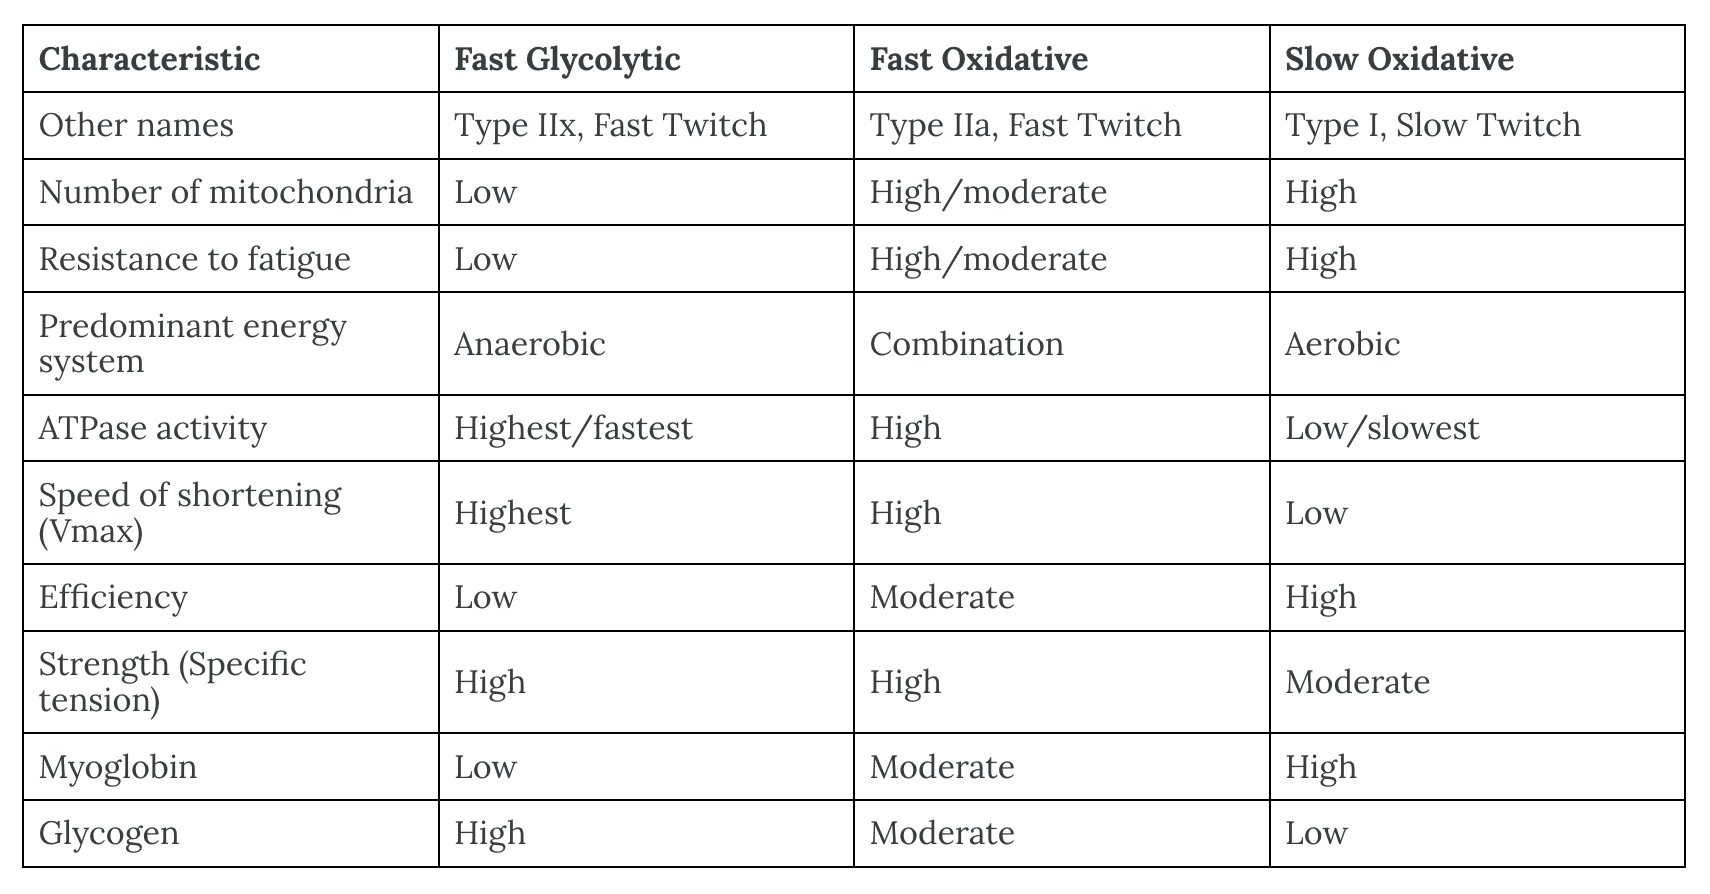
\includegraphics[width=0.9\linewidth]{files/EPpXta8zJdzN048lz8AR-567ef09ff4b90fa51e2af0e3c5e177bf.png}
\caption[]{Summary of muscle fiber types and their characteristics. Image credit: Anatomy \& Physiology Copyright \textcopyright  2019 by Lindsay M. Biga, Staci Bronson, Sierra Dawson, Amy Harwell, Robin Hopkins, Joel Kaufmann, Mike LeMaster, Philip Matern, Katie Morrison-Graham, Kristen Oja, Devon Quick, Jon Runyeon, OSU OERU, and OpenStax. Retrieved from: \href{https://open.oregonstate.education/aandp/chapter/10-5-types-of-muscle-fibers/}{https://open.oregonstate.education/aandp/chapter/10-5-types-of-muscle-fibers/}}
\label{n9KlNIgbBP}
\end{figure}

\subsubsection{At the neural level}

Fatigue does not just occur at the level of muscle fibers, but also has a neural component \citep{taylor2016neural}. Evidence shows that MU firing rates, which are determined by neural activity, decrease during a MVC. Importantly, the use of maximal effort is crucial here, since inconsistent effects across MUs, or even increases in firing rates, can be seen when the percent effort exerted is lower. \citet{taylor2016neural} write, ``\dotsfatigue-induced reductions in firing rates are due to one or a combination of a decline in neural drive, local intrinsic adaptations of the motoneuron\dots, or peripheral inhibitory feedback mechanisms'' (). While an in-depth examination of each of these factors is beyond our scope here (see ), we explain them briefly and how they might affect fatigue.

The first factor --- neural drive --- refers to the signals (in the form of synaptic input) that the MN receives from higher-order brain regions like the motor cortex. During a voluntary contraction, motor `commands' originate in the motor cortex and travel via the corticospinal tract to the MNs in the spinal cord \citep{natali}. MNs then transmit these signals to muscles \citep{}Figure \%s ``. Thus, a change in input to the MN will result in a change in MU firing output. Investigating changes in neural drive during fatigue is not trivial, and studies have shown mixed results. While some studies indicate a decrease in neural drive during MVCs, other studies indicate increases in neural activity \citep{taylor2016neural}, which could suggest compensation for declining activity in the MN and/or muscle.

\begin{figure}[!htbp]
\centering
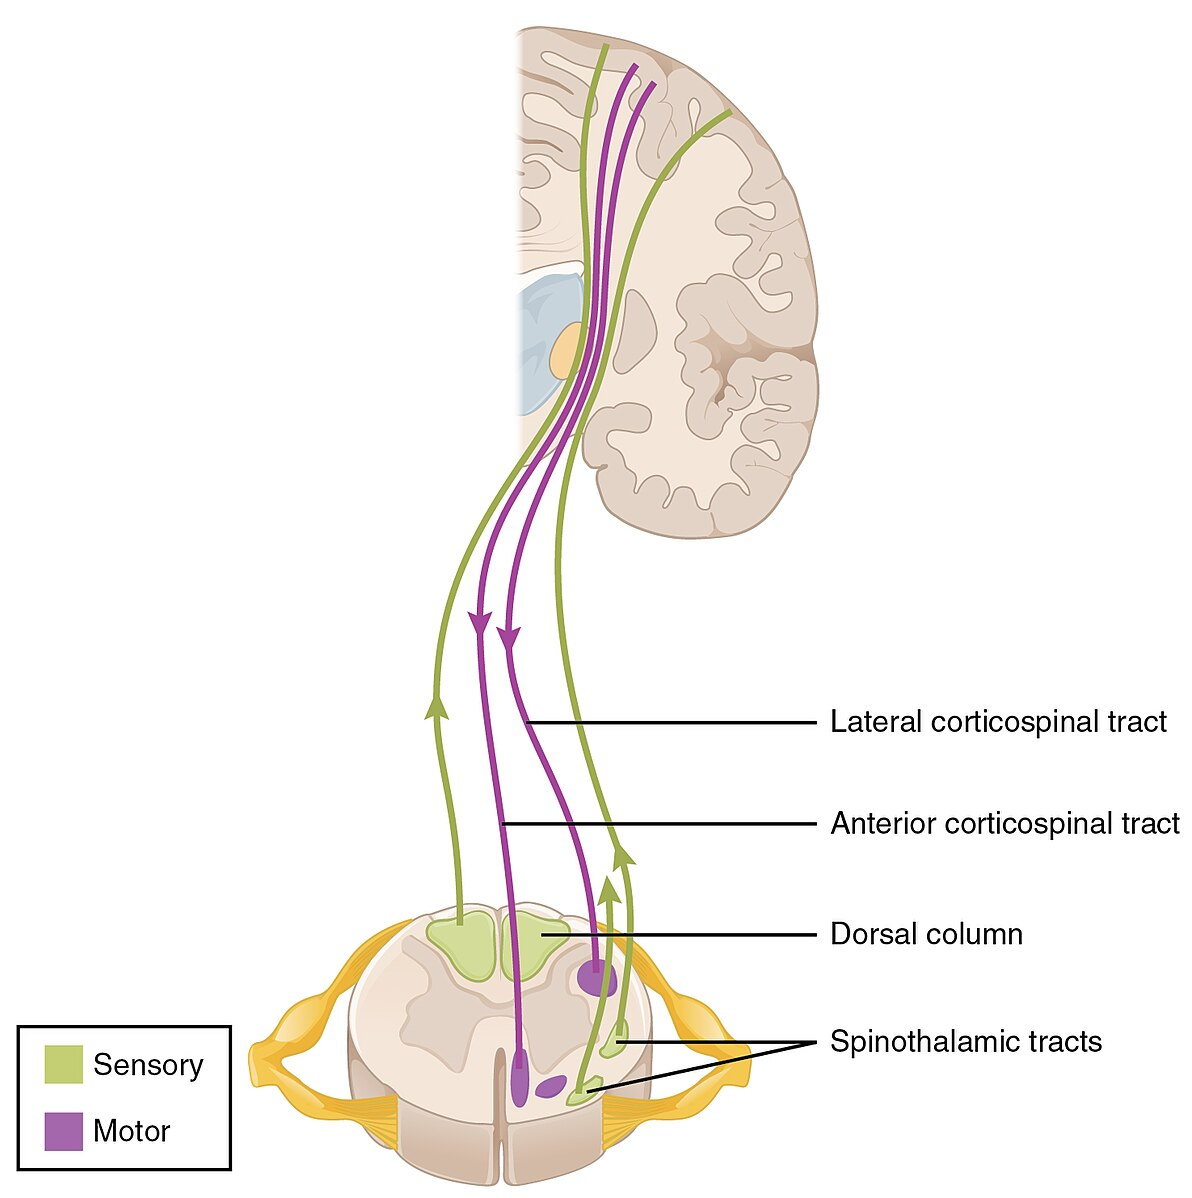
\includegraphics[width=0.7\linewidth]{files/EPpXta8zJdzN048lz8AR-2f1fa6b1e3e30668e32932a0d8625d34.jpeg}
\caption[]{Diagram showing select connections between the brain and spinal cord. The purple line labelled `motor' represents a simplified version of the corticospinal tract by which voluntary motor commands are sent from the motor cortex to the MNs in the spinal cord. Image credit: OpenStax College, CC BY 3.0, via Wikimedia Commons \href{https://upload.wikimedia.org/wikipedia/commons/4/40/1615\_Locations\_Spinal\_Fiber\_Tracts.jpg}{https://upload.wikimedia.org/wikipedia/commons/4/40/1615\_Locations\_Spinal\_Fiber\_Tracts.jpg}}
\label{v9sdMy2gYd}
\end{figure}

In contrast to the extrinsic factor that is neural drive, local intrinsic adaptations refer to processes that occur within the MN itself. These could include a variety of changes, including inactivation of certain channel populations important for MN firing (i.e. less `push'), or a build-up of internal calcium which in turn activates other channels that slow MN firing (i.e. more `brakes'). For an in-depth review of MN properties and channel populations, see \citet{heckman2012motor}.

Finally, the factor `peripheral inhibitory feedback' can be broken down into its component parts. `Peripheral' means that this mechanism originates not in the central nervous system, but instead in the peripheral nervous system, i.e. sensory fibers or receptors found within the skeletal muscles themselves. `Inhibitory feedback', in this case, means that input from these fibers increases as MN activity increases and has the regulatory effect of slowing MN firing (an extrinsic `braking' system). The primary players here are Group III/IV muscle afferents, whose properties and contributions to fatigue are reviewed in \citet{gandevia2001spinal} and \citet{taylor2016neural}.

\subsubsection{Putting it all together}

Muscle fatigue is thus a complex, multifactorial process that involves changes both within and outside the MU. While muscles are fatiguing, cortical drive to MNs may be decreasing; MNs are also decreasing their firing rate due to internal adaptive mechanisms and inhibitory feedback; and finally select muscle fibers are decreasing their responsiveness and eventually dropping out altogether as they fail to produce sufficient energy to maintain contraction. It's not one thing but many that leads to the gradual decrease in force.

\subsubsection{Study questions}

\begin{enumerate}
\item Will you be able to distinguish between the different sources and mechanisms of fatigue in your EMG recordings? If yes, explain how. If no, explain why.
\item Will asking the volunteer to perform a maximal contraction be important for your study? What would you expect to happen if you ask the volunteer to perform contractions with lower or variable percent effort? Explain your answer.
\item Briefly design and describe an experiment to look at the relationship between percent effort and fatigue.
\end{enumerate}

\subsection{Types of muscle contraction}

Fatigue will also depend on the activity being performed. Muscles perform different types of contractions, which generate different levels of force and fatigue. Contractions are often classified as either isometric --- meaning the muscle maintains a constant length ---- or isotonic --- meaning the muscle maintains a constant tension \citep{openStax_neuro}. Within isotonic, contractions can be further divided into concentric, in which the muscle shortens, and eccentric, in which the muscle lengthens \citep{}Figure \%s ``. These classifications can be somewhat misleading for several reasons \citep{faulkner2003terminology}. First, physiological movements typically include combinations of contractions where muscle length and tension vary in time. Thus, most movements, except in controlled experimental settings, are not strictly isometric or isotonic. Second, we can have some shortening of the muscle without necessarily having a change in the joint angle --- an important factor for understanding the tension generated or whether a load was moved (e.g. see the bottom panel in Figure~\ref{OyVvhPkhSg}). For this reason, we'll focus more on the joint angle and carefully design experiments in this practical to try to isolate single movement types.

\begin{figure}[!htbp]
\centering
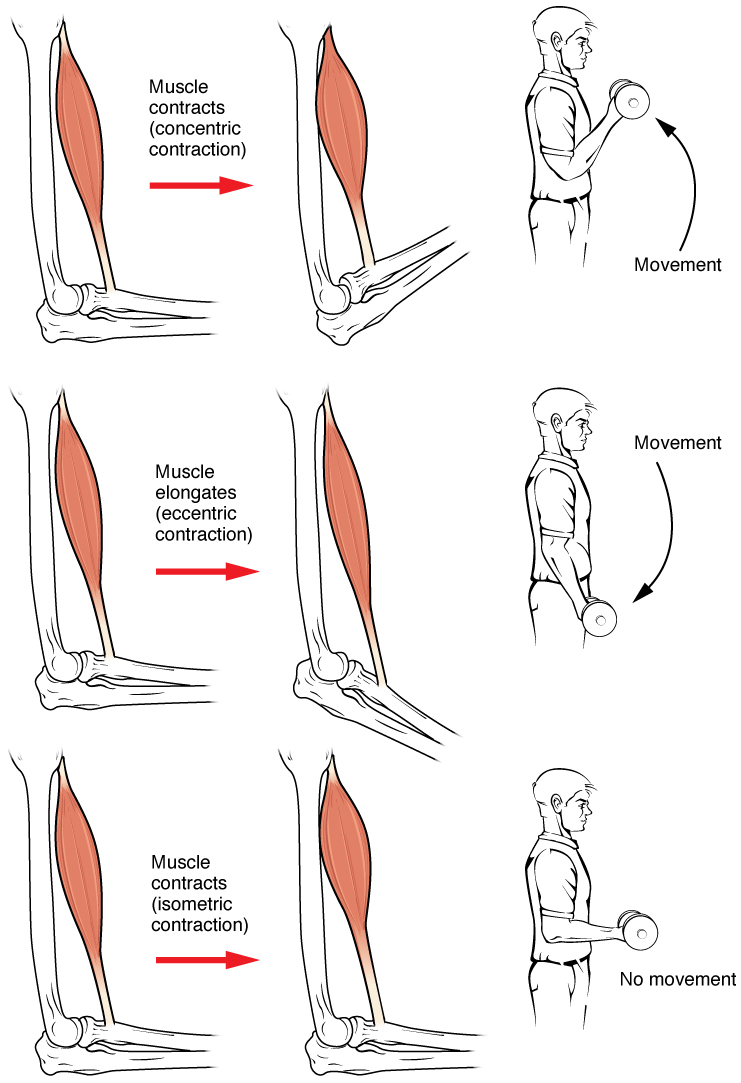
\includegraphics[width=0.5\linewidth]{files/EPpXta8zJdzN048lz8AR-ed134e0857c6a220c0466e6d95d38838.jpeg}
\caption[]{Image credit: OpenStax, CC BY 4.0, via Wikimedia Commons, \href{https://upload.wikimedia.org/wikipedia/commons/d/d4/1015\_Types\_of\_Contraction\_new.jpg}{https://upload.wikimedia.org/wikipedia/commons/d/d4/1015\_Types\_of\_Contraction\_new.jpg}}
\label{OyVvhPkhSg}
\end{figure}

It is generally accepted that eccentric contractions generate the greatest amount of force, followed by isometric, and then concentric contractions \citep{radak2018physiology, feher2017quantitative}. However, results appear mixed on whether eccentric or concentric contractions generate more fatigue, which will likely depend on exactly how exercises are performed and also how fatigue is quantified (e.g. percent change in maximal force versus number of repetitions), among other factors.

\subsubsection{Study questions}

\begin{enumerate}
\item In fatigue tests that involve repeated trials or tests, how will you control for extraneous (non-fatigue related) changes over the course of the experiment? In other words, will the starting conditions for each of your tests always be the same?
\item Will the posture or position of the body during fatigue tests be important? Explain your answer.
\item What variables should you consider when having different volunteers perform the same fatigue test?
\end{enumerate}

\section{Experimental protocol}

Before carrying out this practical, it is recommended that students perform (or at least read through) the `EMG Basics' practical described in Chapter 1. This will help familiarize them with the recording equipment and software. Carry out the steps in stage 1 and 2 of the Ch. 1 experimental protocol to set up the recording device and test the EMG recordings before beginning the fatigue protocols described below.

\subsection{Sustained and repeated isometric contractions}

\begin{enumerate}
\item Place two surface electrodes over the bicep muscle, in parallel with the muscle fibers, and one on the back of the hand or wrist to serve as the reference/ground
\item Ask the volunteer to rest their arm on the table such that they are completely relaxed and the muscle is not generating tension
\item Record the EMG with the muscle at rest for 60 seconds (s); save the recording with a file name to indicate it is the initial control trial
\item On the next trial, ask the volunteer to remain at rest for the first 5 s of the recording, then tense their bicep as much as they can (Maximum Voluntary Contraction) for 50 s, and finally, relax their muscle for the remaining 5 s; stop the recording at 60s
\item The volunteer should rest 30 s before initiating the next trial
\item Repeat step 4 between 5 and 10 times, depending on the level of fatigue, always resting 30 s in between each trial; label the files with the trial number so their order is known
\item Fatigue can be analyzed both within and across trials (see Ch. 5)
\item Think about how you would repeat this protocol but for muscles other than the biceps, both large and small
\end{enumerate}

\subsection{Repeated concentric contractions with load}

\begin{enumerate}
\item Place two surface electrodes over the bicep muscle, and one on the back of the hand or wrist to serve as the reference/ground; if recording from the same volunteer as in Section~\ref{UmjcfszrGT}, allow for appropriate rest and recovery time before starting this protocol
\item Ask the volunteer to test out a few different weights/loads to determine which is appropriate based on their strength; we want the weight to be light enough that they can perform repeated contractions, but not so light that it fails to fatigue the muscle; we also do not want to overload the muscle and cause injury
\item Ask the volunteer to stand up for all trials so as not to impede load movement and minimize compensation from other muscles
\item Record the EMG with the muscle at rest for 60 seconds (s); save the recording with a file name to indicate it is the initial control trial
\item On the next trial, ask the volunteer to remain at rest for the first 5 s of the recording, then ask them to repeatedly lift and lower the load every few seconds for at least 10 repetitions, and finally, relax their muscle for the remaining 5 s; stop the recording at 60s
\item Rest 30 s before initiating the next trial
\item Repeat step 5 between 5 and 10 times, depending on the level of fatigue, always resting 30 s in between each trial; label the files with the trial number so their order is known
\item Think about how fatigue might change if the volunteer kept the load in the lifted position for the duration of each trial
\end{enumerate}

\subsection{Sustained eccentric contraction with load}

\begin{enumerate}
\item Place two surface electrodes over the bicep muscle, and one on the back of the hand or wrist to serve as the reference/ground; if recording from the same volunteer as in previous experiments, allow for appropriate rest and recovery time
\item Ask the volunteer to test out a few different weights/loads to determine which is appropriate based on their strength; note that the weight they can sustain in an eccentric contraction will likely be different from the load they can lift in a concentric contraction
\item Ask the volunteer to stand up for all trials so as not to impede arm position, which will need to be extended out in front of the body
\item Record the EMG with the muscle at rest for 60 seconds (s); save the recording with a file name to indicate it is the initial control trial
\item On the next trial, ask the volunteer to remain at rest for the first 5 s of the recording, then hold the load with their arm extended and the elbow at an angle of 130-135\textsuperscript{o}for 50 s, and finally, relax their muscle for the remaining 5 s; stop the recording at 60s
\item Rest 30 s before initiating the next trial
\item Repeat step 5 between 5 and 10 times, depending on the level of fatigue, always resting 30 s in between each trial; label the files with the trial number so their order is known
\item Think about how you would perform eccentric contractions for muscles other than the bicep
\end{enumerate}

\clearpage
\bibliography{main.bib}

\end{document}
